% Options for packages loaded elsewhere
% Options for packages loaded elsewhere
\PassOptionsToPackage{unicode}{hyperref}
\PassOptionsToPackage{hyphens}{url}
\PassOptionsToPackage{dvipsnames,svgnames,x11names}{xcolor}
%
\documentclass[
  letterpaper,
  DIV=11,
  numbers=noendperiod]{scrartcl}
\usepackage{xcolor}
\usepackage{amsmath,amssymb}
\setcounter{secnumdepth}{5}
\usepackage{iftex}
\ifPDFTeX
  \usepackage[T1]{fontenc}
  \usepackage[utf8]{inputenc}
  \usepackage{textcomp} % provide euro and other symbols
\else % if luatex or xetex
  \usepackage{unicode-math} % this also loads fontspec
  \defaultfontfeatures{Scale=MatchLowercase}
  \defaultfontfeatures[\rmfamily]{Ligatures=TeX,Scale=1}
\fi
\usepackage{lmodern}
\ifPDFTeX\else
  % xetex/luatex font selection
\fi
% Use upquote if available, for straight quotes in verbatim environments
\IfFileExists{upquote.sty}{\usepackage{upquote}}{}
\IfFileExists{microtype.sty}{% use microtype if available
  \usepackage[]{microtype}
  \UseMicrotypeSet[protrusion]{basicmath} % disable protrusion for tt fonts
}{}
\makeatletter
\@ifundefined{KOMAClassName}{% if non-KOMA class
  \IfFileExists{parskip.sty}{%
    \usepackage{parskip}
  }{% else
    \setlength{\parindent}{0pt}
    \setlength{\parskip}{6pt plus 2pt minus 1pt}}
}{% if KOMA class
  \KOMAoptions{parskip=half}}
\makeatother
% Make \paragraph and \subparagraph free-standing
\makeatletter
\ifx\paragraph\undefined\else
  \let\oldparagraph\paragraph
  \renewcommand{\paragraph}{
    \@ifstar
      \xxxParagraphStar
      \xxxParagraphNoStar
  }
  \newcommand{\xxxParagraphStar}[1]{\oldparagraph*{#1}\mbox{}}
  \newcommand{\xxxParagraphNoStar}[1]{\oldparagraph{#1}\mbox{}}
\fi
\ifx\subparagraph\undefined\else
  \let\oldsubparagraph\subparagraph
  \renewcommand{\subparagraph}{
    \@ifstar
      \xxxSubParagraphStar
      \xxxSubParagraphNoStar
  }
  \newcommand{\xxxSubParagraphStar}[1]{\oldsubparagraph*{#1}\mbox{}}
  \newcommand{\xxxSubParagraphNoStar}[1]{\oldsubparagraph{#1}\mbox{}}
\fi
\makeatother


\usepackage{longtable,booktabs,array}
\newcounter{none} % for unnumbered tables
\usepackage{calc} % for calculating minipage widths
% Correct order of tables after \paragraph or \subparagraph
\usepackage{etoolbox}
\makeatletter
\patchcmd\longtable{\par}{\if@noskipsec\mbox{}\fi\par}{}{}
\makeatother
% Allow footnotes in longtable head/foot
\IfFileExists{footnotehyper.sty}{\usepackage{footnotehyper}}{\usepackage{footnote}}
\makesavenoteenv{longtable}
\usepackage{graphicx}
\makeatletter
\newsavebox\pandoc@box
\newcommand*\pandocbounded[1]{% scales image to fit in text height/width
  \sbox\pandoc@box{#1}%
  \Gscale@div\@tempa{\textheight}{\dimexpr\ht\pandoc@box+\dp\pandoc@box\relax}%
  \Gscale@div\@tempb{\linewidth}{\wd\pandoc@box}%
  \ifdim\@tempb\p@<\@tempa\p@\let\@tempa\@tempb\fi% select the smaller of both
  \ifdim\@tempa\p@<\p@\scalebox{\@tempa}{\usebox\pandoc@box}%
  \else\usebox{\pandoc@box}%
  \fi%
}
% Set default figure placement to htbp
\def\fps@figure{htbp}
\makeatother





\setlength{\emergencystretch}{3em} % prevent overfull lines

\providecommand{\tightlist}{%
  \setlength{\itemsep}{0pt}\setlength{\parskip}{0pt}}



 


\KOMAoption{captions}{tableheading}
\usepackage{pdfpages}
\usepackage{graphicx}
\usepackage{eso-pic}
\usepackage{tocloft}
\renewcommand{\cfttoctitlefont}{\Huge\bfseries}
\renewcommand{\cftaftertoctitle}{\vspace{1cm}}
\renewcommand{\cftsecfont}{\fontsize{13pt}{15pt}\selectfont\bfseries}
\renewcommand{\cftsecpagefont}{\fontsize{13pt}{15pt}\selectfont\bfseries}
\setlength{\cftbeforesecskip}{18pt}
\setlength{\cftsecindent}{0pt}
\renewcommand{\cftsubsecfont}{\large}
\renewcommand{\cftsubsecpagefont}{\large}
\setlength{\cftbeforesubsecskip}{12pt}
\setlength{\cftsubsecindent}{1.5em}
\renewcommand{\cftsubsubsecfont}{\normalsize}
\renewcommand{\cftsubsubsecpagefont}{\normalsize}
\setlength{\cftbeforesubsubsecskip}{8pt}
\setlength{\cftsubsubsecindent}{3em}
\makeatletter
\@ifpackageloaded{caption}{}{\usepackage{caption}}
\AtBeginDocument{%
\ifdefined\contentsname
  \renewcommand*\contentsname{Table of contents}
\else
  \newcommand\contentsname{Table of contents}
\fi
\ifdefined\listfigurename
  \renewcommand*\listfigurename{List of Figures}
\else
  \newcommand\listfigurename{List of Figures}
\fi
\ifdefined\listtablename
  \renewcommand*\listtablename{List of Tables}
\else
  \newcommand\listtablename{List of Tables}
\fi
\ifdefined\figurename
  \renewcommand*\figurename{Figure}
\else
  \newcommand\figurename{Figure}
\fi
\ifdefined\tablename
  \renewcommand*\tablename{Table}
\else
  \newcommand\tablename{Table}
\fi
}
\@ifpackageloaded{float}{}{\usepackage{float}}
\floatstyle{ruled}
\@ifundefined{c@chapter}{\newfloat{codelisting}{h}{lop}}{\newfloat{codelisting}{h}{lop}[chapter]}
\floatname{codelisting}{Listing}
\newcommand*\listoflistings{\listof{codelisting}{List of Listings}}
\makeatother
\makeatletter
\makeatother
\makeatletter
\@ifpackageloaded{caption}{}{\usepackage{caption}}
\@ifpackageloaded{subcaption}{}{\usepackage{subcaption}}
\makeatother
\usepackage{bookmark}
\IfFileExists{xurl.sty}{\usepackage{xurl}}{} % add URL line breaks if available
\urlstyle{same}
% fallback for those not using the hyperref driver hyperxmp:
\makeatletter
\@ifundefined{xmpquote}{\newcommand{\xmpquote}[1]{#1}}{}
\makeatother
\hypersetup{
  colorlinks=true,
  linkcolor={blue},
  filecolor={Maroon},
  citecolor={Blue},
  urlcolor={Blue},
  pdfcreator={LaTeX via pandoc}}


\author{}
\date{}
\begin{document}


\includepdf[pages=-]{page_garde_removed.pdf}
\clearpage

\renewcommand*\contentsname{Table des matières}
{
\setcounter{tocdepth}{3}
\tableofcontents
}

\newpage

\section{Introduction}\label{introduction}

Depuis plusieurs années, le numérique a profondément transformé la
manière dont nous consommons et partageons nos loisirs culturels. Le
cinéma dispose de Letterboxd, la musique de Last.fm : des plateformes
communautaires qui permettent à chacun de garder une trace de ses
découvertes, de les noter et d'échanger avec d'autres passionnés. La
lecture, pourtant, reste étonnamment mal servie sur ce plan. Le
principal service existant, Goodreads, appartient à Amazon, ce qui pose
des questions en matière d'indépendance éditoriale et d'exploitation des
données personnelles des lecteurs.

C'est de ce constat qu'est né le projet Ex-Libris : une application de
suivi de lecture pensée comme un véritable réseau social pour les
lecteurs. L'objectif n'est pas de reconstruire un catalogue de livres,
un travail déjà accompli et maintenu par la plateforme collaborative
Open Library, qui référence plusieurs millions d'ouvrages en accès
libre. Ce qu'Open Library ne propose pas, en revanche, c'est la
dimension humaine de la lecture : qui a lu quel livre, quand, avec quel
avis, et quelles recommandations peuvent en être tirées. C'est
précisément cette couche que notre application vient ajouter.

Concrètement, Ex-Libris doit permettre à un utilisateur de créer un
compte, de rechercher un livre et d'en consulter la fiche détaillée, de
l'ajouter à sa bibliothèque personnelle avec un statut de lecture, de le
noter et d'en rédiger une critique. Au-delà de cette gestion
individuelle, l'application intègre une dimension sociale : chaque
utilisateur peut consulter le profil d'un autre lecteur, s'abonner à son
activité, et bénéficier d'un système de recommandation construit à
partir des affinités entre utilisateurs.

D'un point de vue technique, le projet repose sur une API REST
développée avec FastAPI, exploitant les données de l'API publique Open
Library et s'appuyant sur une base de données PostgreSQL pour la
persistance des données propres à notre application. Le langage retenu
est Python, dans une logique de programmation orientée objet.

Ce dossier présente dans un premier temps le cahier des charges du
projet, les choix et arbitrages qui ont guidé nos réflexions, ainsi que
l'organisation retenue au sein de notre équipe. Il détaille ensuite le
modèle de conception élaboré pour répondre à ces besoins, à travers les
différents diagrammes UML réalisés.

\newpage

\section{Cahier des Charges}\label{cahier-des-charges}

Ce cahier des charges exprime le besoin initial auquel notre application
doit répondre : une application de suivi de lecture combinant la
richesse du catalogue d'Open Library à une véritable dimension sociale
entre lecteurs. Sur cette base, notre travail a consisté à reformuler ce
besoin, à en préciser le périmètre exact, et à définir les
fonctionnalités attendues ainsi que les contraintes techniques qui en
découlent, notamment celles liées à l'exploitation d'une source de
données externe que nous ne maîtrisons pas.

\subsection{Présentation d'Open
Library}\label{pruxe9sentation-dopen-library}

\begin{flushright}
\vspace{-1cm}

\includegraphics[width=0.15\textwidth]{OL_logo.png}
\end{flushright}

Notre application repose entièrement sur les données fournies par Open
Library, une base collaborative et gratuite qui référence plusieurs
millions d'ouvrages. Il s'agit d'une API web : on l'interroge en
construisant des adresses (URLs) spécifiques, et elle nous renvoie les
données demandées au format JSON.

\begin{center}

\includegraphics[width=0.8\textwidth]{API1.png}
\end{center}

Pour bien comprendre comment exploiter ces données, il est essentiel de
saisir la façon dont Open Library organise ses informations. La base
distingue en réalité trois notions différentes qui, dans le langage
courant, sont toutes désignées par le mot ``livre'' :

\begin{itemize}
\tightlist
\item
  L'auteur (Author) : la personne ayant écrit l'œuvre.
\item
  L'œuvre (Work) : il s'agit de l'idée générale du livre, indépendamment
  de toute édition particulière. C'est à ce niveau que l'on trouve par
  exemple le titre, un résumé, ou les grands thèmes abordés.
\item
  L'édition (Edition) : il s'agit d'une publication précise et
  matérielle de cette œuvre, par exemple une édition Harcourt de 1971.
  Une même œuvre peut avoir des centaines d'éditions différentes
  (traductions, rééditions, formats poche\ldots).
\end{itemize}

Dans notre base de données, nous avons fait le choix de conserver, pour
chaque œuvre, l'ensemble de ses éditions, afin d'offrir aux utilisateurs
une réelle variété de choix (langue, édition, format) lorsqu'ils
ajoutent un livre à leur bibliothèque. Nous détaillerons la façon dont
nous avons stocké et traité ces données dans la suite de ce dossier
d'analyse, lors de la conception de la maquette.

Nous avons également constaté que certaines données présentes dans Open
Library manquent de cohérence, notamment les thèmes et genres associés
aux œuvres (champ subjects), qui sont rédigés en texte libre et
mélangent parfois de véritables genres littéraires avec de simples
mots-clés. Cette hétérogénéité a directement motivé l'une de nos
réflexions pour la fonctionnalité de normalisation des genres, qui vise
à proposer une classification plus cohérente et plus facilement
exploitable pour la recherche par genre.

\begin{center}

\begin{minipage}{0.45\textwidth}
\centering

\includegraphics[width=\textwidth]{work.png}
\end{minipage}
\hfill
\begin{minipage}{0.45\textwidth}
\centering

\includegraphics[width=\textwidth]{edition.png}
\end{minipage}

\vspace{0.3cm}


\includegraphics[width=0.6\textwidth]{auteur.png}

\end{center}

\newpage

\subsection{Diagramme de cas
d'utilisation}\label{diagramme-de-cas-dutilisation}

\begin{center}

\includegraphics[width=0.62\textwidth]{cas_usage.png}

Figure 11 – Diagramme de cas d'utilisation
\end{center}

\newpage

\subsection{Diagramme d'activité}\label{diagramme-dactivituxe9}

\newpage

\section{Organisation du projet}\label{organisation-du-projet}

\subsection{Organisation du groupe}\label{organisation-du-groupe}

Dès le début du projet, nous avons désigné Anne-Camille Tampet comme
cheffe de projet et Cécile Locatelli comme leader technique, en
veillant, conformément aux conseils donnés en début de projet à ne pas
cumuler ces deux rôles sur une même personne.

Pour communiquer, nous avons créé un groupe sur Teams, sur lequel chacun
peut partager ses avancées, poser une question ou signaler un point de
blocage dès que le besoin s'en fait sentir. C'est notre principal canal
d'échange, sur lequel nous discutons régulièrement. En parallèle, nous
avons mis en place un dépôt partagé sur GitHub, accessible à tous les
membres du groupe, qui nous sert à centraliser et à distribuer
l'ensemble des fichiers importants du projet.

Concernant la répartition du travail, notre organisation a surtout été
pensée pour cette première phase d'analyse. Chaque membre du groupe
s'est vu confier la réalisation d'un diagramme ou d'une partie
spécifique du dossier, de façon à ce que chacun puisse s'investir
concrètement dans la réflexion et la conception du projet. Cette
répartition individuelle ne nous a cependant pas empêchés de travailler
de façon très collective. Nous avons pris l'habitude de nous retrouver
au minimum deux fois par semaine pour faire le point ensemble. Ces
moments nous permettaient de relire et de discuter les diagrammes
réalisés par chacun, de nous assurer que tout le monde comprenait bien
les choix faits par les autres et de les faire évoluer si nécessaire.
Cette phase de discussion collective a été particulièrement importante
en tout début de projet. Elle nous a permis de poser une base commune
solide et de nous assurer que tout le monde partageait la même vision de
l'application avant d'avancer plus en détail sur la partie codage.

\begin{center}

\includegraphics[width=0.62\textwidth]{git.png}

Figure 11 – Dépot Github
\end{center}

\subsection{Diagramme de Gantt}\label{diagramme-de-gantt}

\begin{center}

\includegraphics[width=0.8\textwidth]{Gantt.png}

Figure 11 – Diagramme de Gantt
\end{center}

Notre planning se découpe en deux grandes phases. D'abord la phase
d'analyse, de fin août à fin septembre : nous commençons par étudier
l'API Open Library, puis nous réalisons l'ensemble de la modélisation
UML afin de bien comprendre comment notre application va s'articuler et
comment la construire.

Une fois cette base posée, nous passons à la phase de code, d'octobre à
début novembre. Nous avons choisi de développer les fonctionnalités par
ordre de difficulté croissante : d'abord les classes de base, puis
l'authentification et la recherche de livres (F1-F2), la bibliothèque
avec les statuts de lecture (F3), les critiques (F4), et enfin notre
fonctionnalité F5 (les recommandations), qui nécessitera davantage de
temps du fait de sa complexité. Les tests unitaires et le frontend
interviendront en dernier, le frontend n'étant pas prioritaire, sera
développé uniquement s'il nous reste du temps.

\newpage

\section{Maquette de l'application}\label{maquette-de-lapplication}

\subsection{Diagrammes BDD}\label{diagrammes-bdd}

\subsection{Diagramme de classes}\label{diagramme-de-classes}

\subsubsection{Classes Business Object}\label{classes-business-object}

\begin{center}

\includegraphics[width=0.8\textwidth]{Buissiness_object.png}

Figure 11 – Diagramme de classe : Business Object
\end{center}

\subsubsection{Classes DAO}\label{classes-dao}

\subsubsection{Classes Service}\label{classes-service}

\subsection{Diagrammes de séquence}\label{diagrammes-de-suxe9quence}

Les diagrammes de séquence suivant permettent de détailler la
chronologie des échanges entre les différents composants de notre
architecture (Utilisateur, Front End, Back End, DAO, API externe) pour
trois fonctionnalités de l'application : la suppression d'une fiche de
lecture, la sélection d'un livre et la demande de recommandations
personnalisées.

\begin{center}
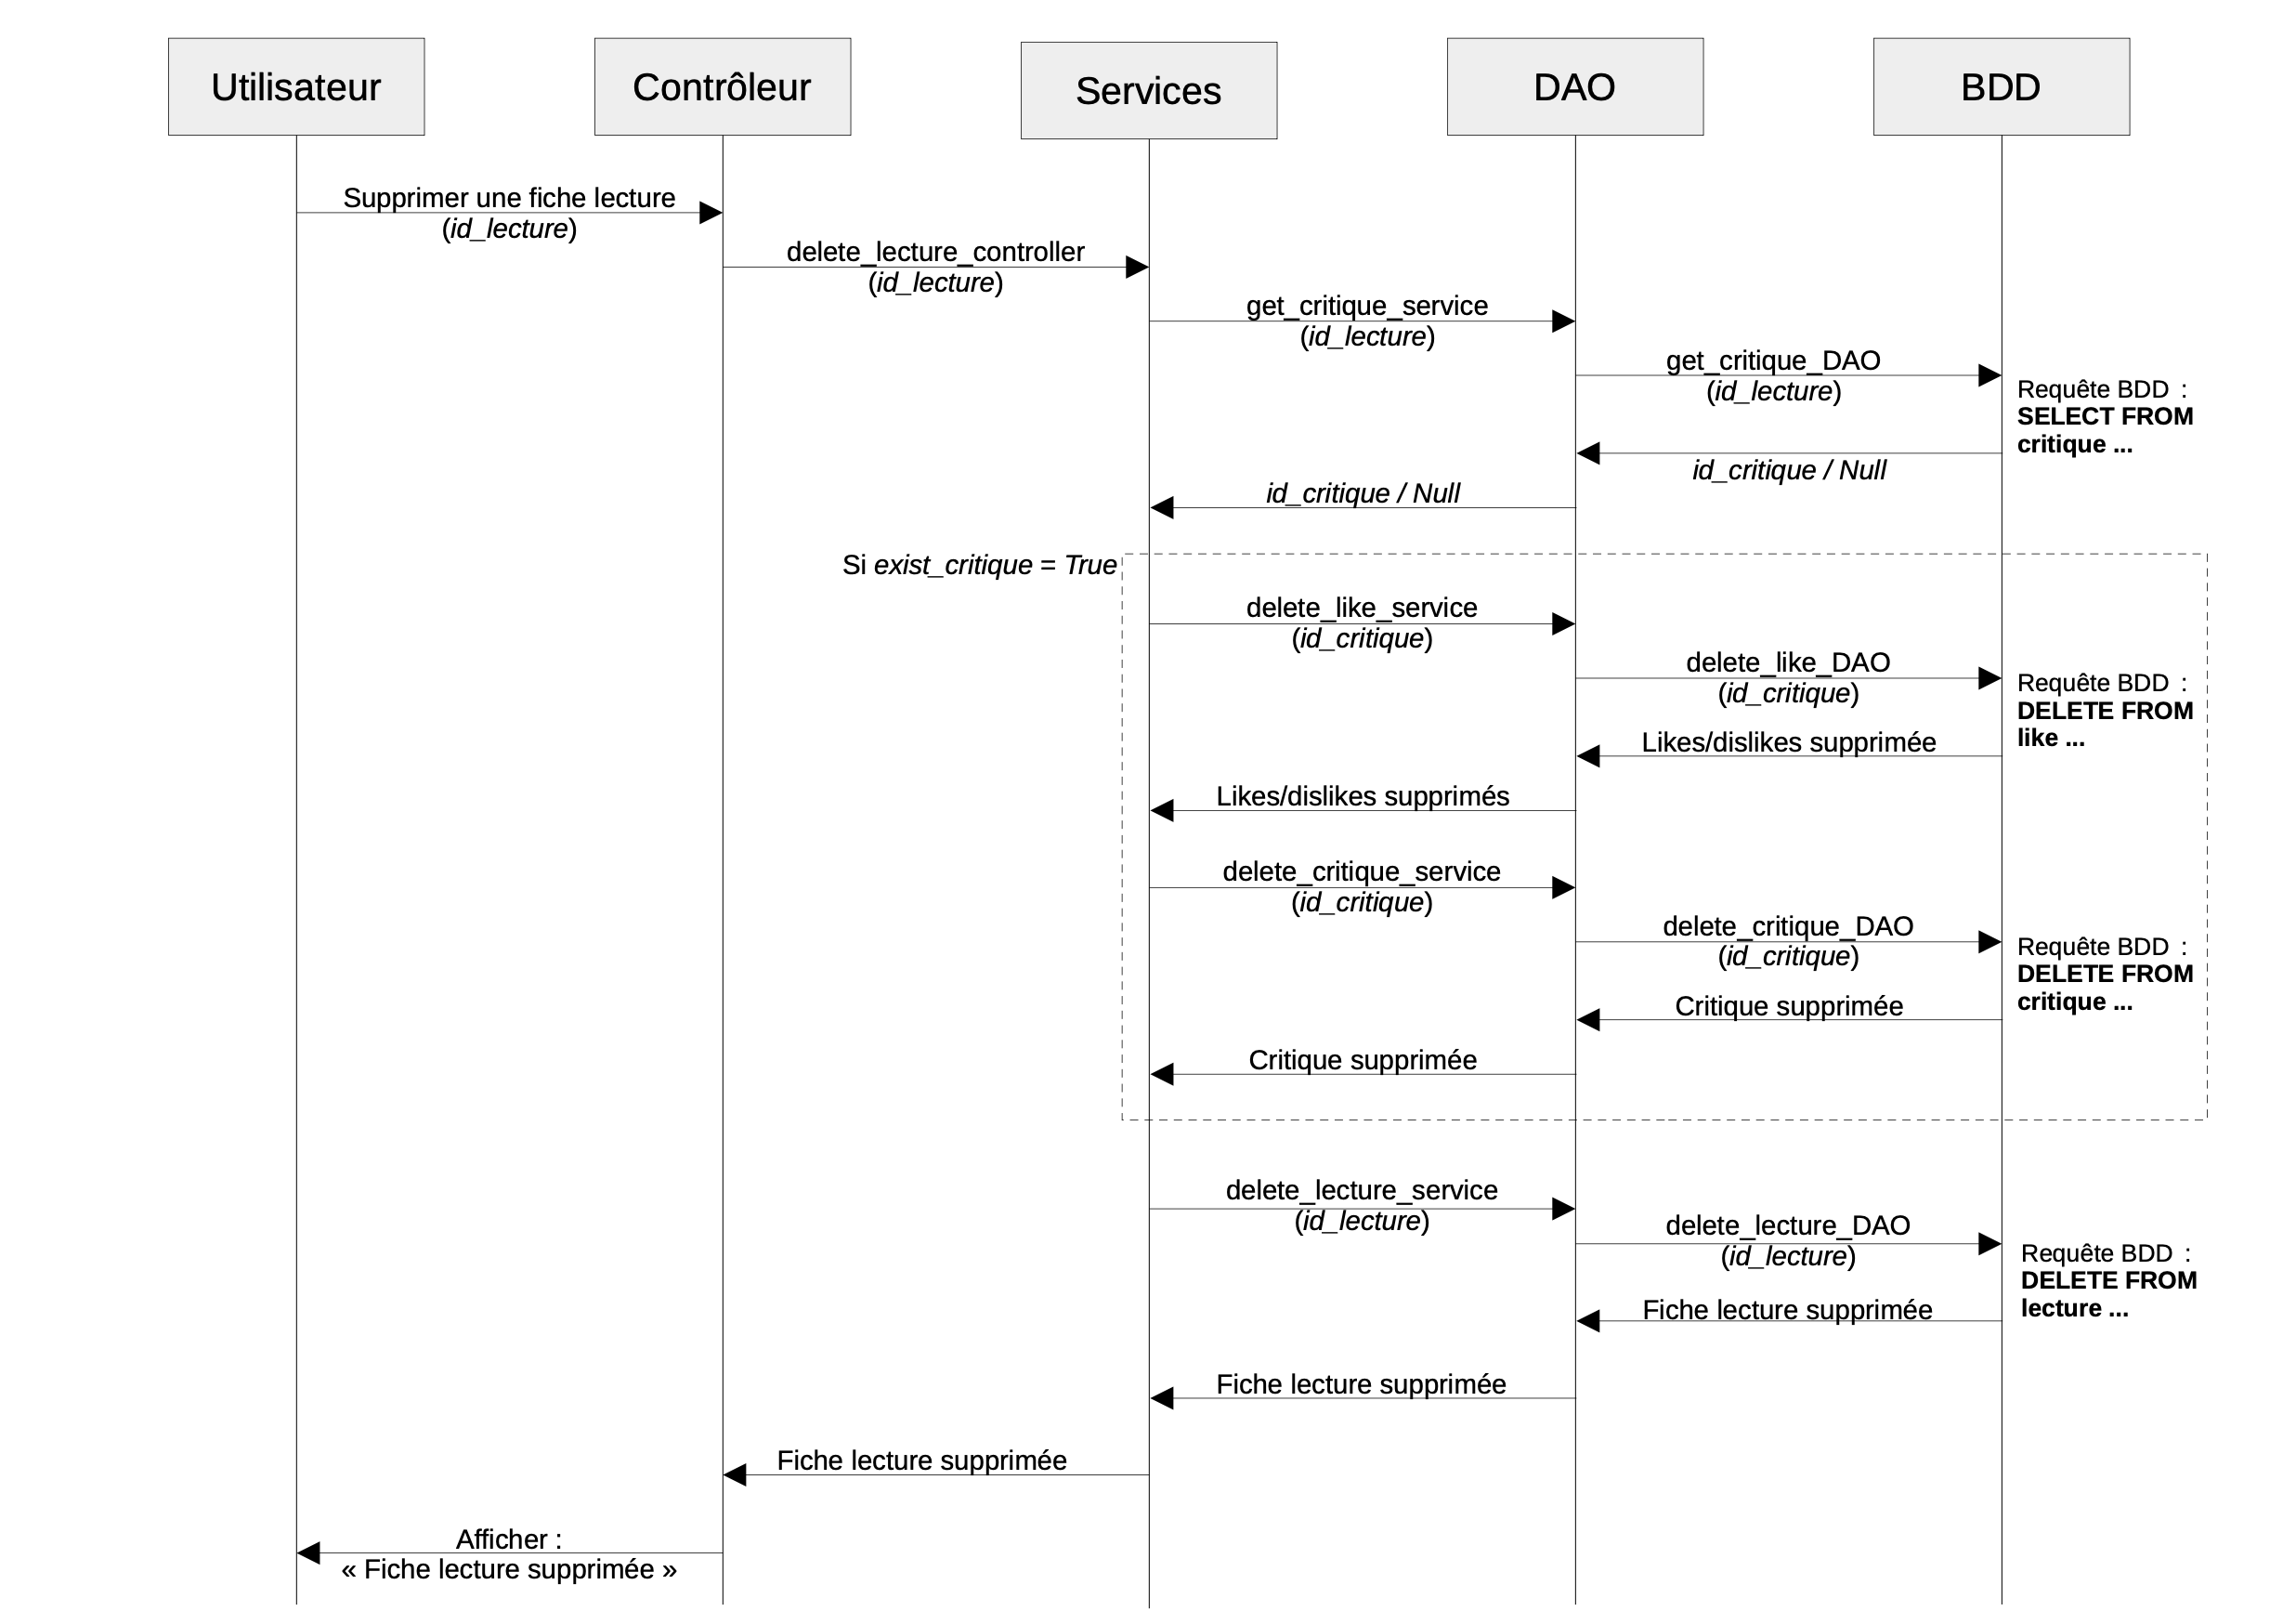
\includegraphics[width=0.6\textwidth]{Diagramme_Séquence_Suppression-fiche-lecture_page-0001.jpg}

Figure 11 – Diagramme de séquence : supprimer une fiche de lecture
\end{center}

Le but de cette séquence est de supprimer une fiche lecture pour un
utilisateur.

Celui-ci a créé auparavant une fiche lecture : il a enregistré un livre
avec des informations (statut du livre, note, etc., il a éventuellement
ajouté une critique associée). Il souhaite aujourd'hui la supprimer.

Il se situe au départ sur la fiche lecture considérée, et clique sur un
bouton « Supprimer la fiche lecture ».

L'information, avec l'id\_lecture (l'identifiant de la fiche lecture)
est réceptionnée par le \textbf{Contrôleur}, qui la transmet au
\textbf{Service}, qui envoie des requêtes au \textbf{DAO}.

Dans un premier temps, la fiche lecture est supprimée de la table de
données « \texttt{lecture} », ainsi que sa note associée.

Ensuite, le \textbf{Service} va rechercher dans la base de données
l'existence éventuelle d'une critique associée à cette lecture. Si une
critique est trouvée, alors celle-ci sera supprimée, ainsi que
d'éventuels likes/dislikes associés.

À la fin de toutes ces opérations, le \textbf{Service} transmet au
\textbf{Contrôleur} l'information que la fiche a bien été supprimée,
celui-ci affiche à l'écran de l'utilisateur « La fiche lecture a bien
été supprimée ».

\begin{center}
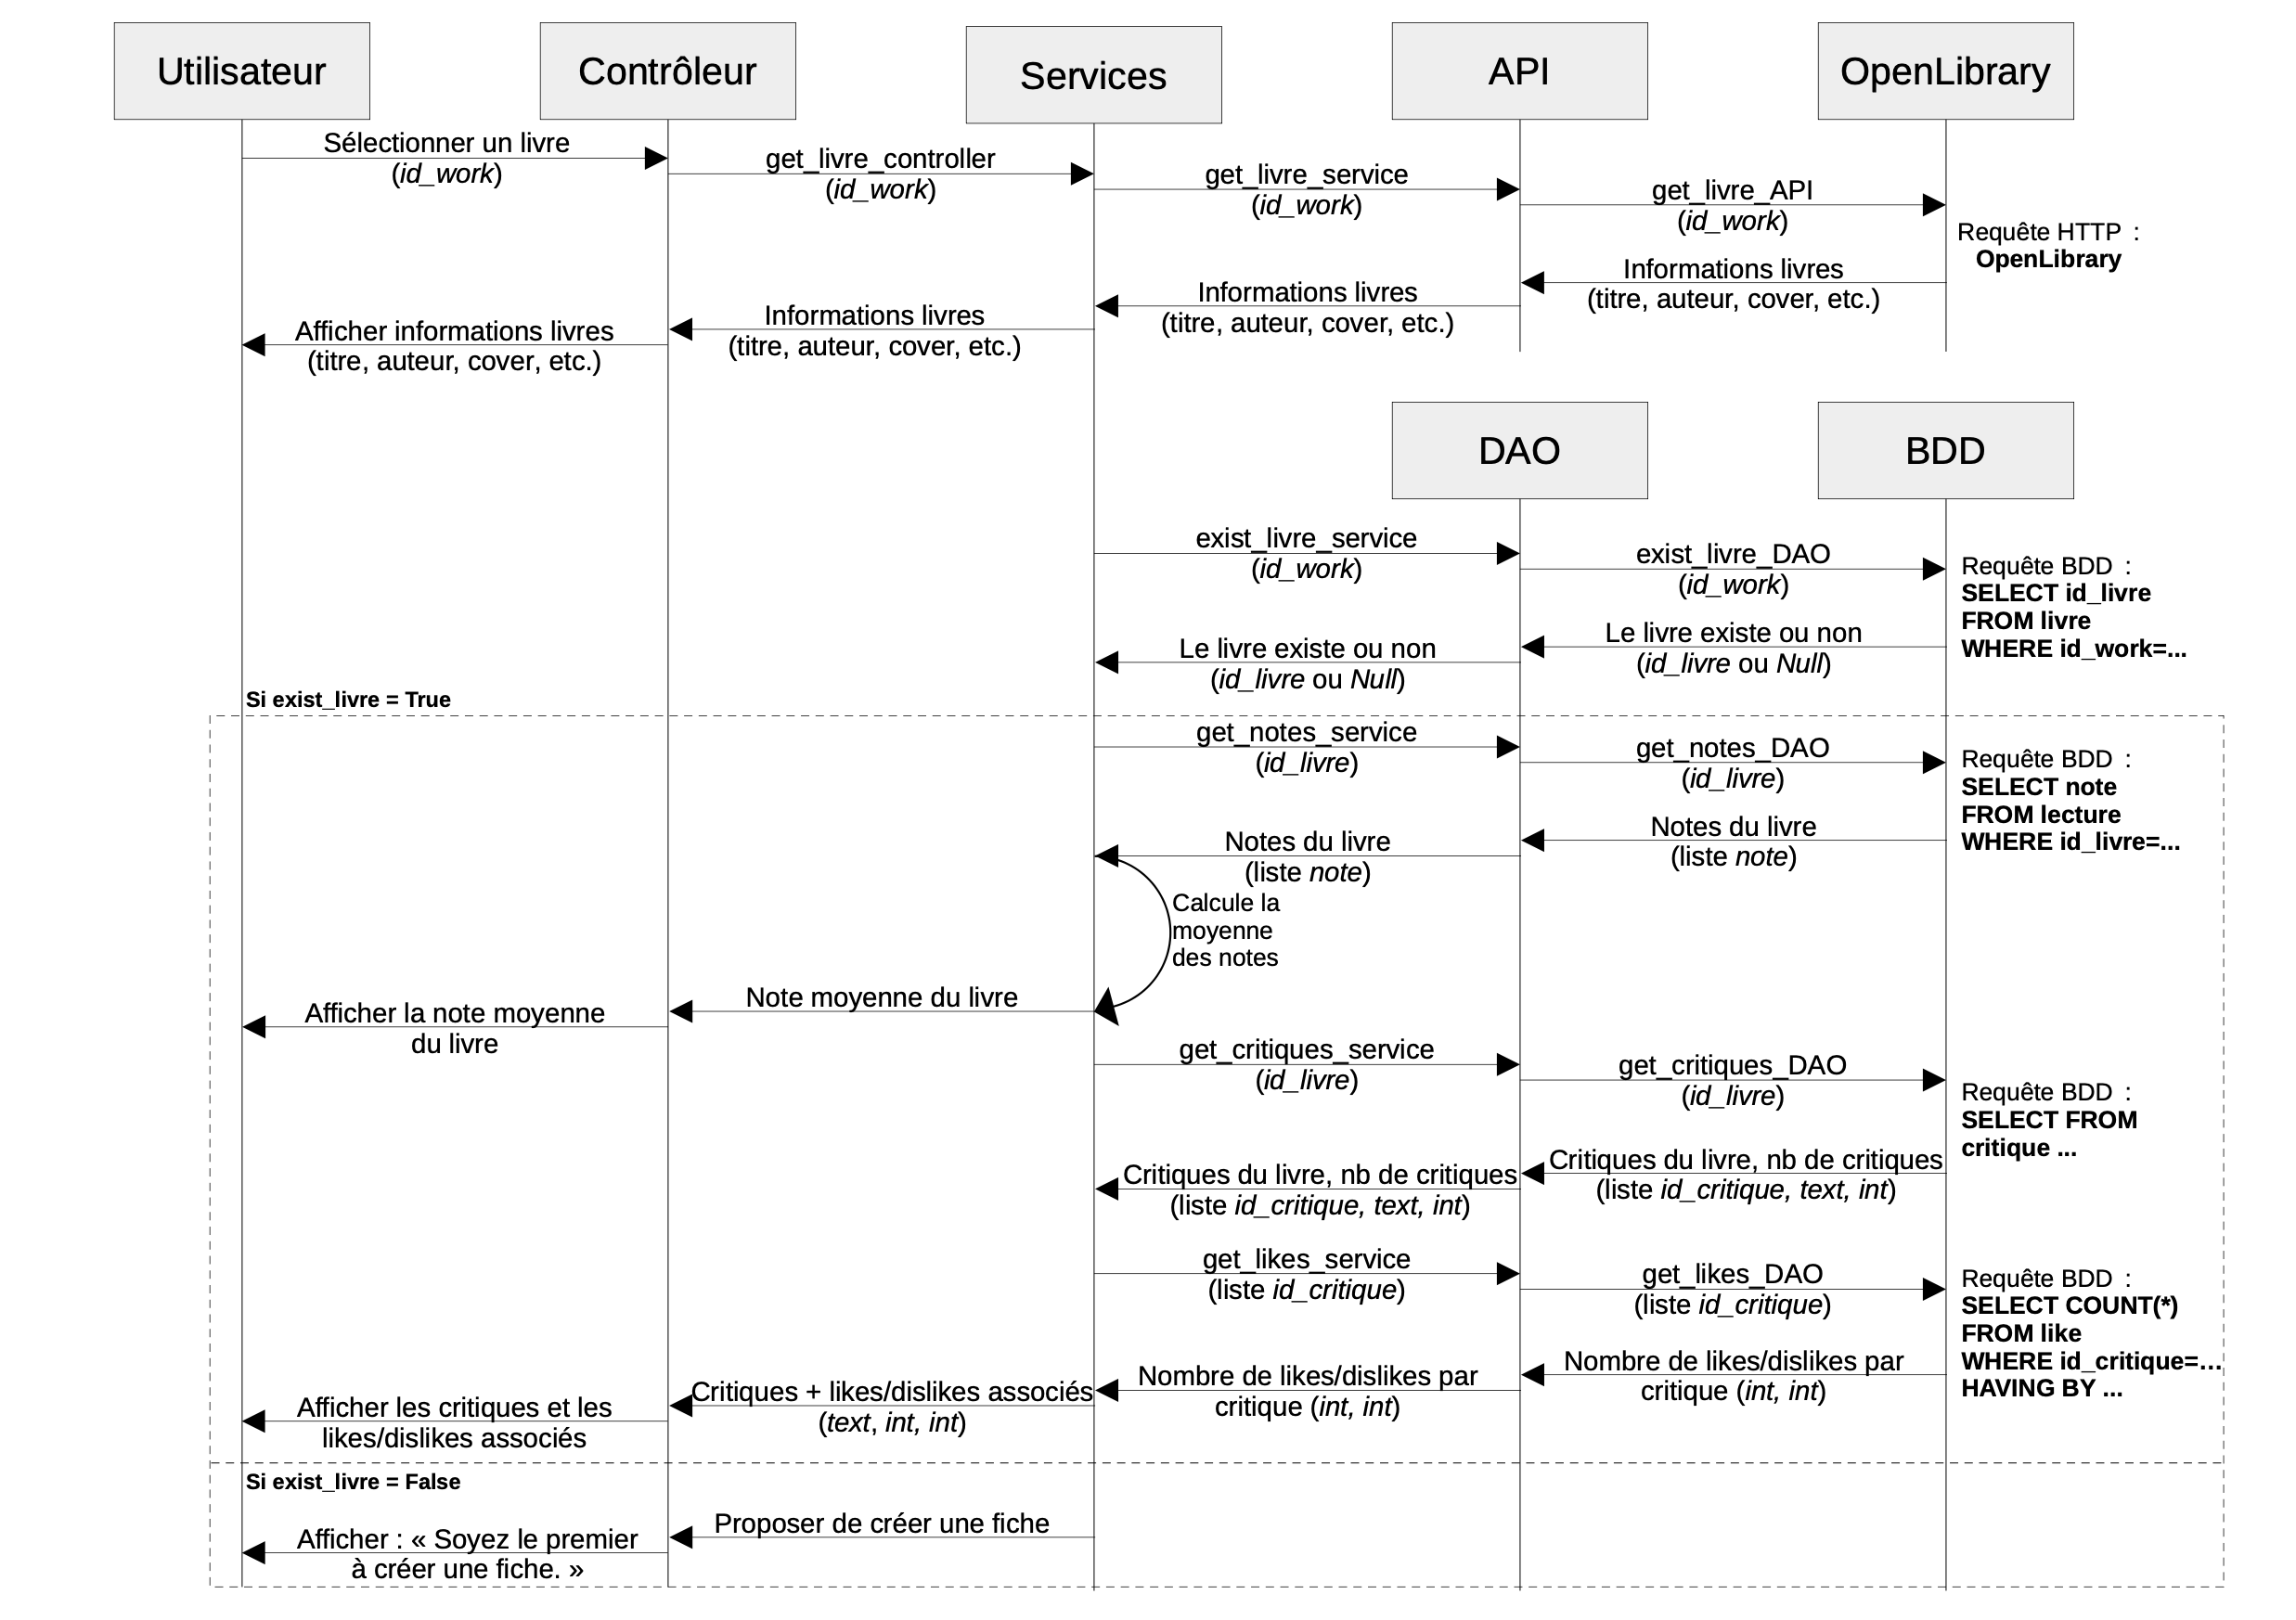
\includegraphics[width=0.58\textwidth]{Diagramme_Séquence_Sélectionner-livre_page-0001.jpg}

Figure 11 – Diagramme de séquence : sélectionner un livre
\end{center}

Ce diagramme décrit l'affichage de la fiche détaillée d'un livre, qui
combine des données externes et des données propres à notre application.
Lorsque l'utilisateur sélectionne un livre, le Back End interroge dans
un premier temps l'API Open Library afin de récupérer les informations
bibliographiques (couverture, sous-titre, etc.) qui ne sont pas stockées
localement. En parallèle, le Back End consulte la DAO pour extraire les
données internes à Ex-Libris associées à ce livre : les fiches de
lecture existantes, les critiques rédigées par les utilisateurs, ainsi
que les likes et dislikes rattachés à chacune d'elles. Une agrégation
est également effectuée côté Back End : les notes attribuées par les
lecteurs sont récupérées puis moyennées pour produire une note globale
du livre. L'ensemble de ces informations (Open Library, critiques,
likes/dislikes, note moyenne) est ensuite consolidé et renvoyé au Front
End pour affichage. Ce diagramme illustre bien la logique de notre
architecture : Open Library reste la source de vérité pour le contenu
bibliographique, tandis que notre base de données ne conserve que ce qui
relève de l'activité des utilisateurs. \vspace{0.4cm}

\begin{center}
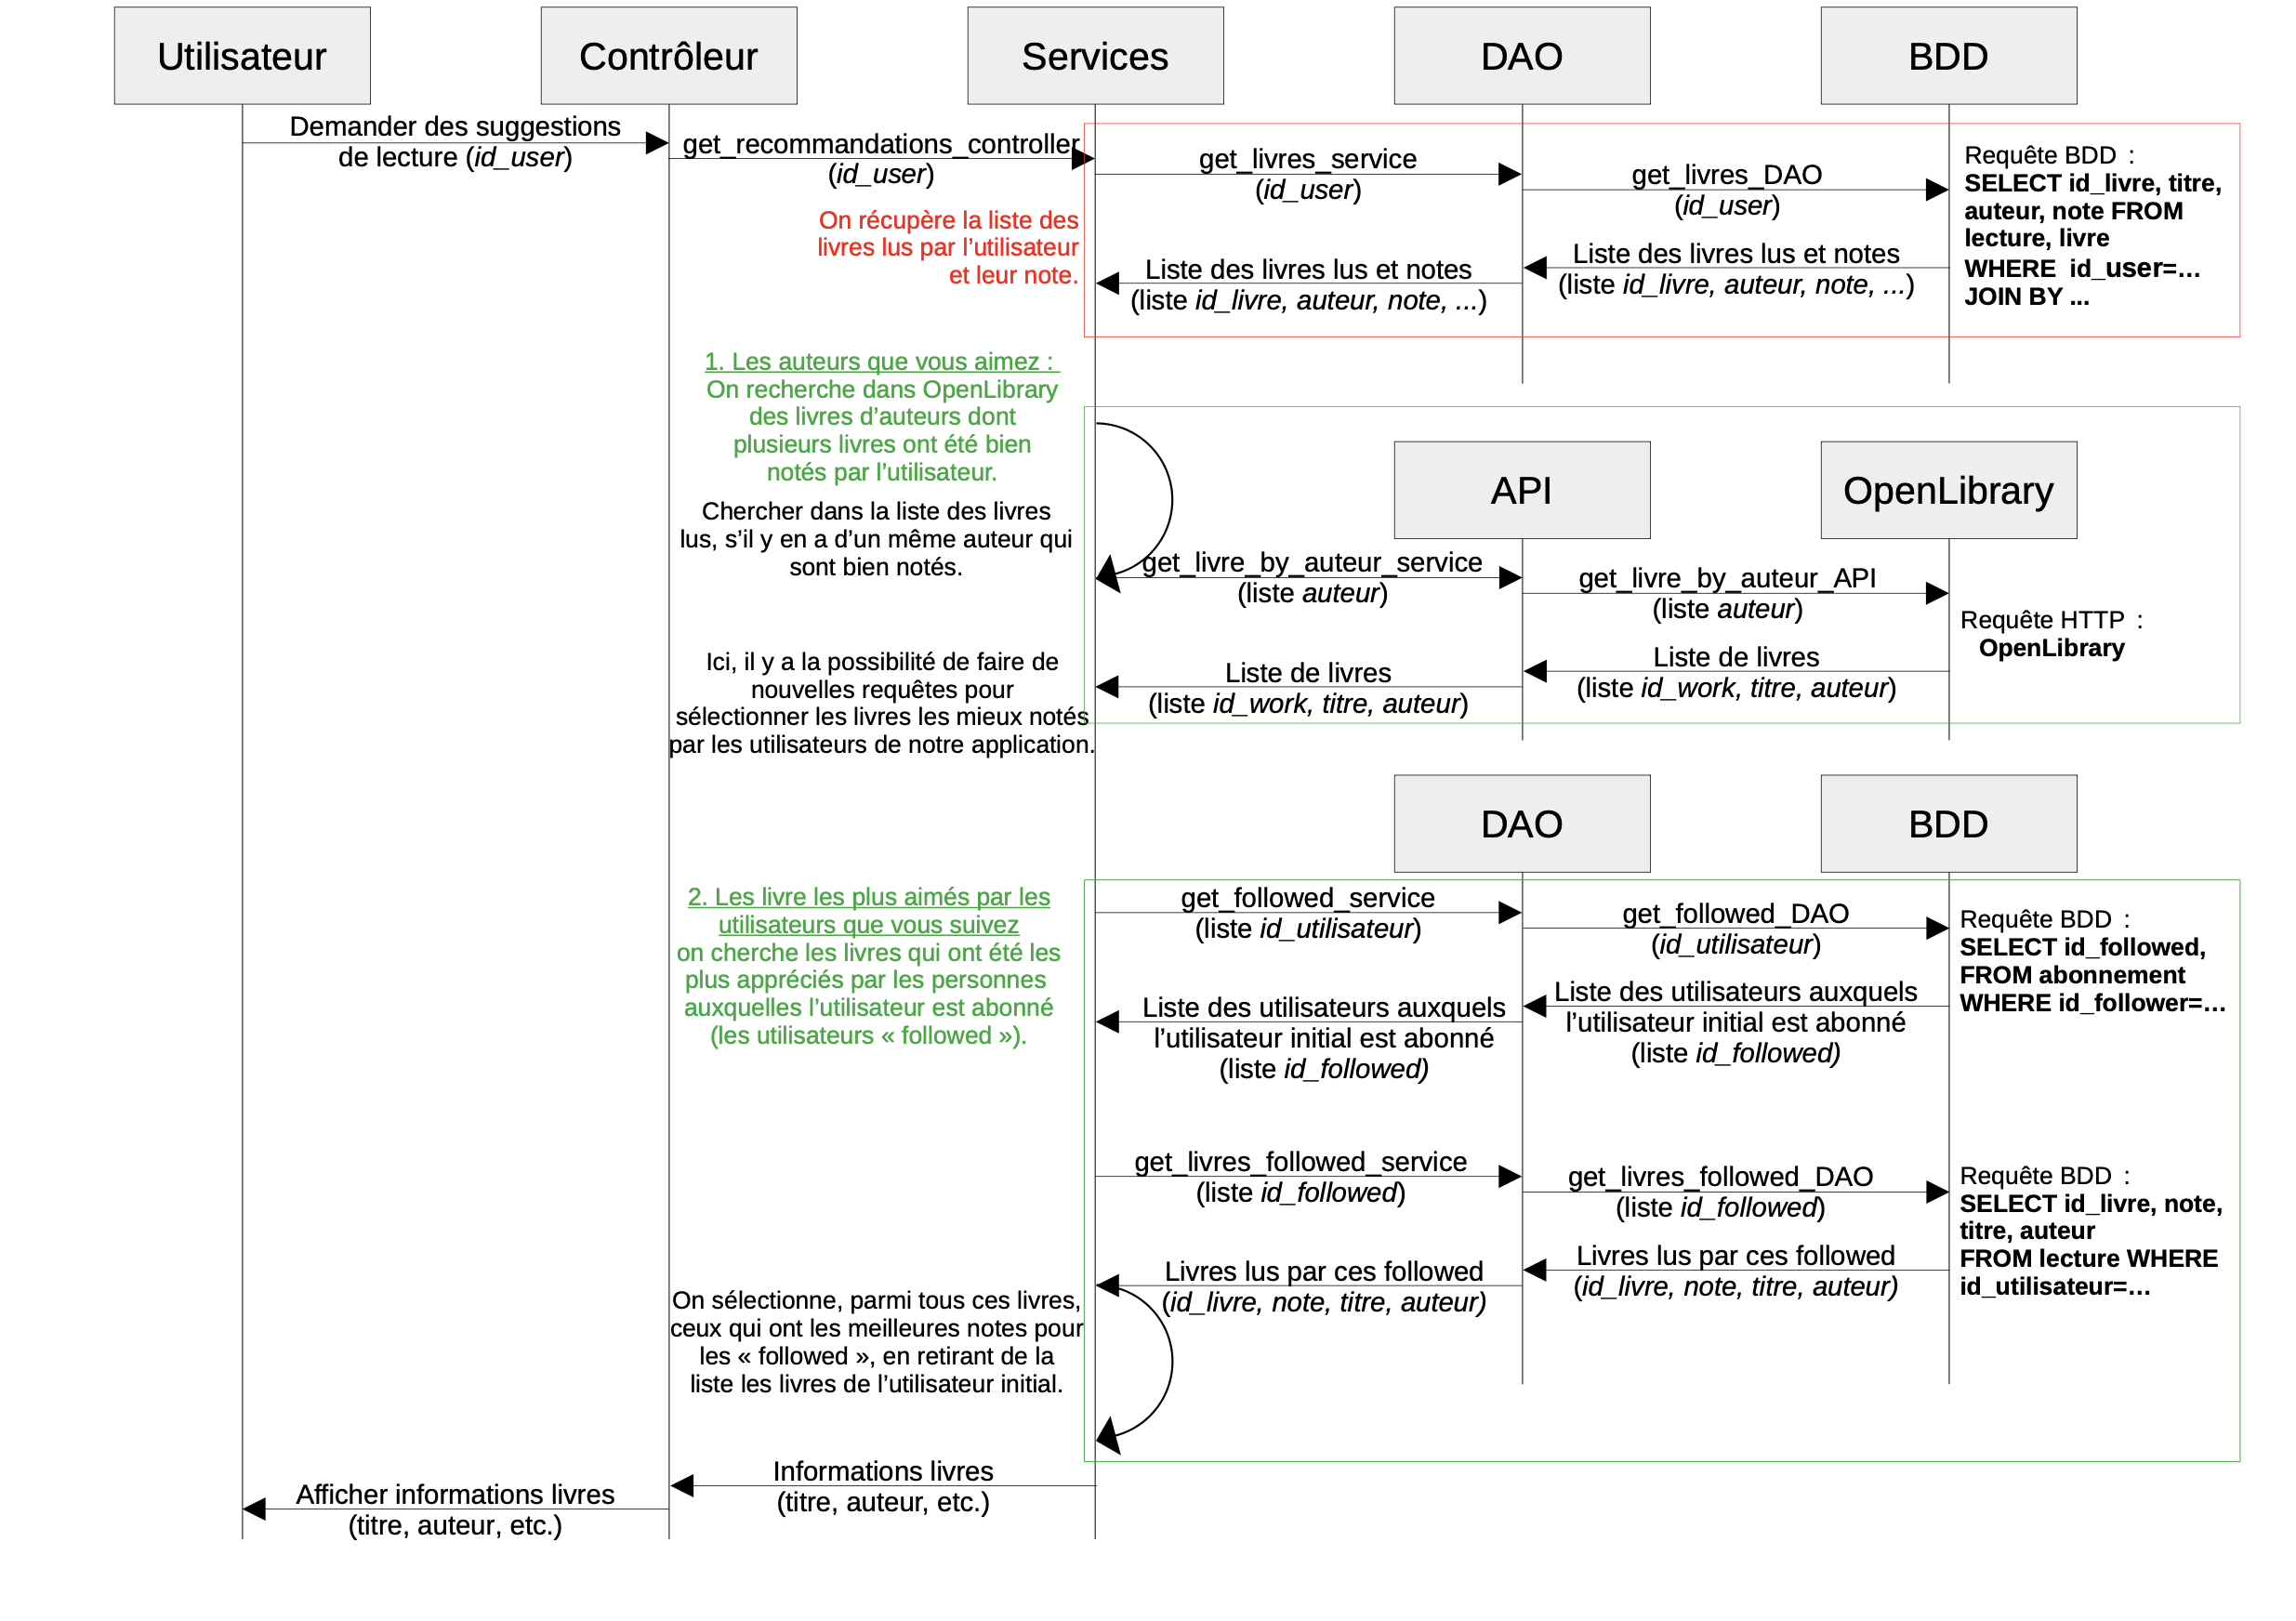
\includegraphics[width=0.58\textwidth]{Diagramme_Séquence_demander-des-recommandations_page-0001.jpg}

Figure 11 – Diagramme de séquence : sélectionner un livre
\end{center}

Ce diagramme correspond à notre fonctionnalité F5, un système de
recommandation basé sur les affinités entre lecteurs. Le processus se
déroule en plusieurs temps. Le Back End récupère d'abord, via la DAO, la
liste des livres déjà lus par l'utilisateur demandeur. Pour chacun de
ces livres, une requête identifie les autres utilisateurs ayant
également lu ce même livre. Le Back End calcule ensuite, lecteur par
lecteur, le nombre de livres en commun avec l'utilisateur initial, ce
qui permet de dégager un sous-ensemble de « lecteurs similaires » selon
un critère de recoupement. Pour ces lecteurs sélectionnés, l'application
récupère l'ensemble de leurs livres lus ainsi que les notes associées.
Le Back End retire alors de cette liste les livres déjà lus par
l'utilisateur initial et ne conserve que les livres les mieux notés ou,
en l'absence de signal suffisant, propose des livres bien notés au
hasard parmi ceux restants. Une fois la sélection finale établie, les
informations bibliographiques des livres recommandés sont récupérées
auprès de l'API Open Library avant d'être affichées à l'utilisateur.

partie 1 : Cahier des Charges partie 2 : Maquette de l'application

📋 Suivi projet Ex-Libris

✅ Fait

\begin{itemize}
\tightlist
\item
  Arno : diagramme de séquence (partie 2)
\item
  Paul : diagramme de Gantt (partie 1) paul le caca qui pue berkkkkk
\item
  Cecile : Diagramme de cas d'utilisation (partie 1)
\end{itemize}

🔄 En cours

\begin{itemize}
\tightlist
\item
  Moussa : diagramme BDD (partie 2)
\item
  Axel : diagramme d'activité (partie 1)
\item
  Anne-Camille : diagramme de classe business (détail + explication des
  classes) (partie 2)
\item
  Paul : Introduction
\end{itemize}

⬜ À faire

\begin{itemize}
\tightlist
\item
  Partie répartition des tâches et présentation de l'équipe (partie 2)
\item
  Diagramme de package (DAO / Services / Business / View) (partie 2)
\item
  Détail d'un service (partie 2)
\item
  Présentation de l'API (partie 1) \ldots{}
\end{itemize}




\end{document}
